\section{Implementazione}

\subsection{Implementazione C} \label{impC}
L'algoritmo è composto da due fasi, il calcolo delle statistiche per ogni permutazione e il confronto dei risultati ottenuti.
Poiché il risultato deve essere un booleano che indica se le popolazioni dispongono delle stesse caratteristiche, e la statistica è indipendente dal test allora ne consegue la intestazione della funzione c può essere la seguente


\begin{lstlisting}[style=CStyle]
int runPermutationTest(Data *data, float (*statistic)(Data* data));
\end{lstlisting}

Data è la struct contenente è definita come segue

\begin{lstlisting}[style=CStyle]

typedef struct data
{	
	float* sample;
	unsigned size;
	unsigned cutPoint;
	float alpha;
	float iterations;
} Data;

\end{lstlisting}

dove sample è il puntatore al primo elemento dell'array dei dati che include entrambe le popolazioni, cutPoint è la dimensione della prima popolazione (e di conseguenza l'indice del primo elemento della seconda) e size è la somma della dimensione del primo campione e del secondo. La dimensione del secondo campione può essere ricavata come size - cutPoint. Alpha è il livello di significatività del test, mentre iterations è il numero di iterazioni da effettuare.

Si noti anche il secondo parametro
\begin{lstlisting}[style=CStyle]
float (*statistic)(Data* data)
\end{lstlisting}

tale scrittura indica che il secondo parametro è una funzione che accetta un puntatore a Data e ritorna un float, cioè una funzione che rappresenta una statistica.

La funzione risulta quindi essere:

\begin{lstlisting}[style=CStyle]

int runPermutationTest(Data *data, float (*statistic)(Data* data))
{
	float statistics[data->iterationsCount];
	
	//calcolo della statistica delle popolazioni non permutate
	float sampleStatistic = statistic(data); 	
	
	//calcolo delle statistiche permutate
	for (unsigned a = 0; a < data->iterations; a++)
	{
		permutate(data);
		statistics[a] = statistic(data);
	}
	
	//confronto della statistica con quelle permutate
	sort(statistics, data->iterations, sizeof(float));
	int k = data->iterations-((int)(data->alpha * data->iterations));	
	return statistics[k] > sampleStatistic;
	
}
\end{lstlisting}

La parte in cui si gestisce il caso statistics[k] == sampleStatistic del return è stato ignorato in favore della semplicità della descrizione. In tali situazioni è sufficiente generare un numero casuale tra 0 e 1 e accettare il risultato se tale valore è inferiore ad alpha. Ciò garantisce che anche nel caso si esegua una permutazione sola il numero di falsi allarmi sarà esattamente alpha.


\paragraph{OpenCL}

Gli ultimi 15 anni hanno visto l'affermarsi della tecnologia delle schede grafiche come strumento utile alla computazione ad alta velocità.
Progettate inizialmente per la creazione di immagini 3D da presentare a schermo, tali unità di calcolo presentano caratteristiche che le rendono adatte a eseguire calcoli in parallelo.
Una scheda grafica è composta svariate unità di calcolo ognuna disposta dei propri registri privati, queste unità sono poi riunite in gruppi i quali condividono una memoria locale e infine tutte loro accedono alla stessa memoria globale. 
I gruppi condividono anche parte delle componenti hardware, in particolare quelle legate al controllo del flusso del programma. Ciò implica che mentre il consumo energetico è minore rispetto alle cpu convenzionali, le unità di calcolo all'interno di un gruppo devono necessariamente eseguire le stesse operazioni. Tale tecnica prende il nome di SIMD, cioè Single Instruction Multiple Data, poiché disponendo di registri diversi per ogni nucleo di calcolo è possibile raggiungere risultati distinti su ognuno di essi, anche se la procedura è la stessa.
\line(1,0){320}

\begin{center}
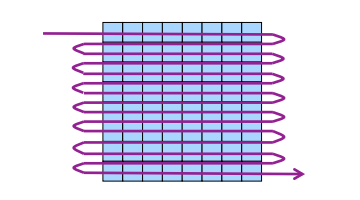
\includegraphics[scale=0.5]{sequential}
\captionof{figure}{Processo Sequenziale}
\end{center}
\begin{center}

	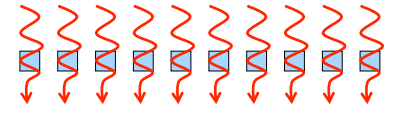
\includegraphics[scale=0.5]{parallel}
	\captionof{figure}{Processo SIMD}
\end{center}

\line(1,0){320}

Tale architettura permette quindi di accelerare tutti gli algoritmi che possono essere eseguiti in parallelo. Questo è esattamente il caso riguardante i permutation test, se si seleziona una statistica adatta, poiché le permutazione non necessitano di conoscere quale fosse stato il risultato della permutazione precedente, mentre i calcolo della statistica segue le stesse operazioni in ogni unità di calcolo.

Si è mostrato come l'implementazione in un linguaggio di programmazione convenzionale risulta essere triviale, discuteremo ora di come implementare tale algoritmo in OpenCL, cioè uno dei linguaggi utilizzati dalle schede grafiche. Un programma OpenCL prende il nome di kernel. Un kernel è fondamentalmente una funzione che viene invocata da un normale programma risiedente nella macchina ospite della scheda. L'invocatore deve specificare quali sono i parametri di invocazione, e quale è l'area memoria dove il kernel può scrivere il risultato computato. 
Inoltre è necessario specificare quante unità di calcolo vogliamo dedicare all'operazione, anche se tale valore non è accessibile all'interno di un programma OpenCl.

Ad esempio supponiamo di voler scrivere un kernel che raddoppia il valore di ogni elemento di un array


\begin{lstlisting}[style=CStyle]
__kernel void double(__global const float *in, __global float *out)
{
	unsigned int i = get_global_id(0);
	
	out[i] = in[i] * 2;
}
\end{lstlisting}

Il programma invocante caricherà nel vettore in i dati da raddoppiare, creerà l'array out dal quale desidera ricavare i risultati e infine lancerà il kernel, indicando che desidera dedicare un numero di core pari alla dimensione dell'array.

Ogni core utilizzerà la funzione get\_global\_id per ricavare il proprio offset rispetto alla prima unità di calcolo e utilizzerà questo valore per scoprire quale numero deve raddoppiare e dove deve essere salvato.

La keyword \_\_global serve per indicare alla scheda che è un riferimento alla memoria condivisa tra tutte le unità di calcolo. 

\subparagraph{Implementazione permutation test}
Per scrivere un algoritmo in OpenCL è necessario identificare quale parti dell'implementazione descritta nella sezione \ref{impC} sono adatti ad essere selezionati per essere svolti in parallelo.

I dati originali vengono ospitati sulla scheda, il ciclo contenuto del ciclo for viene spostato, nel kernel che si desidera scrivere, mentre l'ordinamento e il confronto vengono operati sulla cpu.


Risulta quindi che un kernel è composto dalla permutazione e dalla valutazione della statistica. 

\begin{lstlisting}[style=CStyle]
	__kernel void p_test
	(
	__global const float* in,
	__global float* out,
	unsigned int cutPoint,
	unsigned int sampleSize,
	)
	{
		unsigned int i = get_global_id(0);
		float[sampleSize] permutated;
		
		permutate(in, permutated, i);
		
		b[i] = evaluateStatistic(in, sampleSize, cutPoint, vectorSize);
	}
\end{lstlisting}

La scrittura efficiente della statistica verrà analizzata nella sezione \ref{ottimizzazione}, e l'intero problema si riduce alla capacità di permutare i dati in ingresso.

Ciò è possibile basandosi sulla seguente osservazione:
Sia P un numero primo qualsiasi, allora $$ \forall X, Y  \in [0,  \frac{P}{2} ] :  X \neq Y \Rightarrow (X * X) \% P \neq (Y * Y) \% P.$$
Ciò significa che se due numeri minori di $\frac{P}{2}$ sono diversi allora è diverso il loro quadrato modulo P, e questo garantisce che se i risultati calcolati dalla espressione

$$F(x) = (x * x)\%P$$

non si ripetano mai. Questa proprietà permette di costruire un una funzione biettiva da $[0, P] \Rightarrow [0, P]$ , cioè una permutazione pseudorandomica che opera in tempo e memoria costante.

Il codice risulta quindi essere:
 
\begin{lstlisting}[style=CStyle]
unsigned int singlePermutate(unsigned int x, unsigned int prime)
{	
	if (x <= prime / 2)
		return x * x % prime;
	else
		return prime - (x * x % prime);	

}
\end{lstlisting}

Si noti che alcune ottimizzazioni sono necessarie per rompere la simmetria centrale dovuta al funzionamento della formula, ma verranno tralasciate per semplicità.

Da questa funzione segue che la variabile X rappresenta il seme del generatore di numeri casuali, e quindi è sufficiente a rappresentarne completamente lo stato. 

Il kernel diviene quindi, a patto che sample size sia uguale un numero primo .
\begin{lstlisting}[style=CStyle]
	__kernel void p_test
	(
	__global const float* in,
	__global float* out,
	unsigned int cutPoint,
	unsigned int sampleSize,
	)
	{
		unsigned int i = get_global_id(0);
		float[sampleSize] permutated;
		
		for (int a = 0; a < sampleSize; a++)
			permutated[i] =int[singlePermutate(a, sampleSize)];
		
		b[i] = evaluateStatistic(in, sampleSize, cutPoint, vectorSize);
	}
\end{lstlisting}

Risulta quindi che tutto ciò che rimane da fare è ordinare i risultati e confrontarli con la statistica dei dati non premutati. Tale computazione può essere svolta dal programma risiedente nella memoria principale della macchina, poiché è necessario attendere che tutte le statistiche vengano valutate e nel caso si utilizzasse più di una scheda non vi è alcuna garanzia che esse terminino in contemporanea. 


\subsection{Test Multivariati}
Queste ottimizzazioni riguardano esclusivamente la maniera in cui si accede ai dati depositati nella memoria della scheda. Di conseguenza è possibile caricare dati sotto forma di struct, invece che semplici float. Risulta quindi raggiunto uno degli obiettivi di tale documento, disponiamo di un implementazione di un test di ipotesi capace di operare su campioni multivariati che non necessita di precalcolare le soglie.